% Generated 2020-08-21 17:36:03 +0530
\subsection{Motion} \label{sec:Motion}


\begin{figure}[ht]
  \centering
    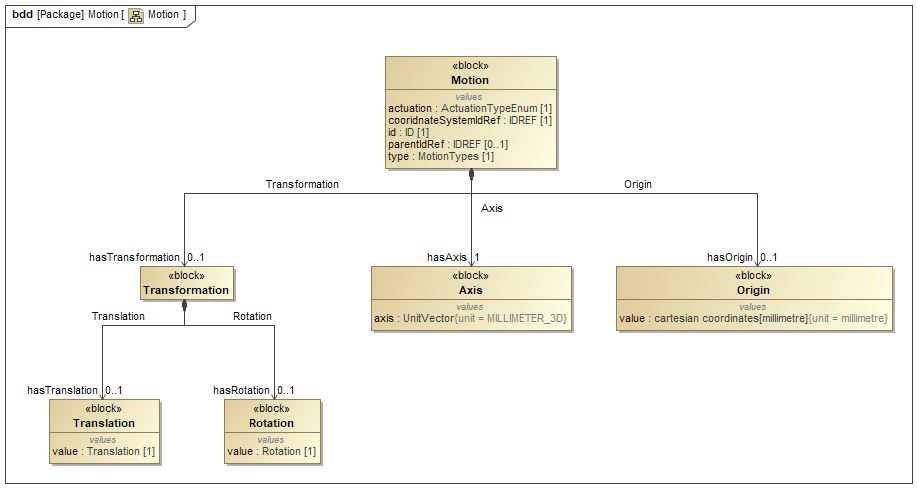
\includegraphics[width=1.0\textwidth]{figures/Motion.png}
  \caption{Motion Diagram}
  \label{fig:Motion}
\end{figure}

\FloatBarrier



\subsubsection{Axis}
\label{sec:Axis}



\block{Axis} defines the axis along or around which the component moves relative to a coordinate system.


\paragraph{Attributes of Axis}\mbox{}
\label{sec:Attributes of Axis}

\tbl{Attributes of Axis} lists the attributes of \texttt{Axis}.

\begin{table}[ht]
\centering 
  \caption{Attributes of Axis}
  \label{table:Attributes of Axis}
\tabulinesep=3pt
\begin{tabu} to 6in {|l|l|l|} \everyrow{\hline}
\hline
\rowfont\bfseries {Attribute} & {Type} & {Multiplicity} \\
\tabucline[1.5pt]{}
\property{axis}[Axis] & \texttt{UnitVector} & 1 \\
\end{tabu}
\end{table}
\FloatBarrier


Descriptions for attributes of \block{Axis}:

\begin{itemize}
\item \property{axis}[Axis] : The unit vector defining the axis of motion.
\end{itemize}
\FloatBarrier

\subsubsection{Motion}
\label{sec:Motion}



\block{Motion} defines the movement of the component relative to a coordinate system. \block{Motion} specifies the kinematic chain of the components.


\paragraph{Attributes of Motion}\mbox{}
\label{sec:Attributes of Motion}

\tbl{Attributes of Motion} lists the attributes of \texttt{Motion}.

\begin{table}[ht]
\centering 
  \caption{Attributes of Motion}
  \label{table:Attributes of Motion}
\tabulinesep=3pt
\begin{tabu} to 6in {|l|l|l|} \everyrow{\hline}
\hline
\rowfont\bfseries {Attribute} & {Type} & {Multiplicity} \\
\tabucline[1.5pt]{}
\property{actuation}[Motion] & \texttt{ActuationTypeEnum} & 1 \\
\property{cooridnateSystemIdRef}[Motion] & \texttt{IDREF} & 1 \\
\property{id}[Motion] & \texttt{ID} & 1 \\
\property{parentIdRef}[Motion] & \texttt{IDREF} & 0..1 \\
\property{type}[Motion] & \texttt{MotionTypes} & 1 \\
\end{tabu}
\end{table}
\FloatBarrier


Descriptions for attributes of \block{Motion}:

\begin{itemize}
\item \property{actuation}[Motion] : Describes if this component is actuated directly or indirectly as a result of other motion.

\tabulinesep = 5pt
\begin{longtabu} to \textwidth {
    |l|X|}
  \caption{ActuationTypeEnum Enumeration}
  \label{enum:ActuationTypeEnum} \\

\hline
Name & Description \\
\hline
\endfirsthead
\hline
\multicolumn{2}{|c|}{Continuation of Table \texttt{ActuationTypeEnum} Enumeration} \\
\hline
Name & Description \\
\hline
\endhead
\texttt{DIRECT} & The movement is initiated by the component. \\ \hline
\texttt{DERIVATIVE} & The movement is derived from other components motion. \\ \hline
\texttt{VIRTUAL} & The motion is computed and is used for expressing an imaginary movement. \\ \hline
\texttt{FIXED} & The component does not move. \\ \hline
\end{longtabu}

\FloatBarrier
\item \property{cooridnateSystemIdRef}[Motion] : The coordinate system within which the kinematic motion occurs.
\item \property{id}[Motion] : The identifier of this element.
\item \property{parentIdRef}[Motion] : The kinematic chain connects all components using the parent relations. All motion is connected to the motion of the parent. The first node in the chain will not have a parent.
\item \property{type}[Motion] : Describes the type of motion.

\tabulinesep = 5pt
\begin{longtabu} to \textwidth {
    |l|X|}
  \caption{MotionTypes Enumeration}
  \label{enum:MotionTypes} \\

\hline
Name & Description \\
\hline
\endfirsthead
\hline
\multicolumn{2}{|c|}{Continuation of Table \texttt{MotionTypes} Enumeration} \\
\hline
Name & Description \\
\hline
\endhead
\texttt{PRISMATIC} & Moves along an axis. \\ \hline
\texttt{REVOLUTE} & Rotates around an axis. \\ \hline
\texttt{TWIST} & Rotates in a twisting motion around an axis. \\ \hline
\texttt{REVOLVE} & Revolves around an axis. \\ \hline
\end{longtabu}

\FloatBarrier
\end{itemize}

\paragraph{Elements of Motion}\mbox{}
\label{sec:Elements of Motion}

\tbl{Elements of Motion} lists the elements of \texttt{Motion}.

\begin{table}[ht]
\centering 
  \caption{Elements of Motion}
  \label{table:Elements of Motion}
\tabulinesep=3pt
\begin{tabu} to 6in {|l|l|l|} \everyrow{\hline}
\hline
\rowfont\bfseries {Element Name} & {Type} & {Multiplicity} \\
\tabucline[1.5pt]{}
\block{Axis} & \texttt{Axis} & 1 \\
\block{Origin} & \texttt{Origin} & 0..1 \\
\block{Transformation} & \texttt{Transformation} & 0..1 \\
\end{tabu}
\end{table}
\FloatBarrier


Descriptions for elements of \block{Motion}:

\begin{itemize}
\item \block{Axis} : \block{Axis} defines the axis along or around which the component moves relative to a coordinate system.
\item \block{Origin} : The coordinates of the origin position of a coordinate system.
\item \block{Transformation} :  The process of transforming to the origin position of the coordinate system from a parent coordinate system using \block{Translation} and \block{Rotation}.
\end{itemize}
\FloatBarrier
